\acresetall
\chapter{Learning and Memory}
\label{ch:intro:memory}
\section*{Overview}
Learning and memory define who we are and shape who we will become.
The various components of memory -- learning, adaptation, plasticity, association, conditioning -- are fundamental features of nervous systems across all organisms.
Indeed, humanity's greatest adaptation is perhaps our unparalleled ability to learn from and adapt to the world around us.
The study of memory in the brain spans from the level of molecular changes that occur at synapses between individual cells to the role of entire brain regions in facilitating different components of memory.
% Over time, our understanding of memory has evolved from the earliest quantifications of the limits of human memory \citep{Ebbinghaus1885} to a molecular understanding of the changes within the brain that occur following learning \citep{Kandel2001}.

In the following sections I aim to describe an understanding of memory, the brain structures underlying it, and cellular physiological correlates of learning relevant to my later studies.
In discussing learning and memory, I will first focus on spatial memory as a core component of episodic memory (\autoref{sec:intro:memory:memory}) and how we experimentally study it.
While learning-related changes are fundamental to every neuron in the nervous system, I will primarily focus on the role of the \ac{HPC} in learning and memory, as the \ac{HPC} is most relevant to the memory systems I will be studying (\autoref{sec:intro:memory:structure}).
Finally, I will discuss our current understanding of cellular and circuit mechanisms by which the brain encodes and recalls memory, with a specific emphasis on hippocampal place cells underlying spatial memory (\autoref{sec:intro:memory:physiology}).

\section{Memory}
\label{sec:intro:memory:memory}
Memory is the way in which experiences from the past can influence how we interpret the present (or the future).
Memory includes explicit memories of objects, concepts, people, places, and events (\textsc{declarative memory}), but also skills and abilities that we cannot consciously recall, such as the ability to shoot a basketball or ride a bike (\textsc{implicit memory}).
% Forms of implicit memory are evolutionarily ancient, present in the earliest invertebrates \citep{Milner1998}.
Declarative memory can be subdivided into at least two categories: autobiographical episodic memory of events and general knowledge of facts, known as semantic memory.
As Endel Tulving explained when he defined \textsc{episodic memory}, these two memory systems are not entirely independent:

\begin{quote}
Episodic memory retrieves and stores information about temporally dated episodes or events, and temporal-spatial relations among these events. A perceptual event can be stored in the episodic system solely in terms of its perceptible properties or attributes, and it is always stored in terms of its autobiographical reference to the already existing contents of the episodic memory store. The act of retrieval of information from the episodic memory store, in addition to making the retrieved contents accessible to inspection, also serves as a special type of input into episodic memory and thus changes the contents of the episodic memory store. The system is probably quite susceptible to transformation and loss of information. While the specific form in which perceptual input is registered into the episodic memory can at times be strongly influenced by information in semantic memory--we refer to the phenomenon as encoding--it is also possible for the episodic system to operate relatively independently of the semantic system.
\attrib{\citealt[pgs.~385-386]{Tulving1972}}
\end{quote}

This interpretation of episodic memory encapsulates several key points that I will address going forward.
The time and space at which an event occurred are essential components of the memory -- they are the relationship framework that we use to categorize events in memory (\autoref{sec:intro:memory:spatial-episodic}).
Also, episodic memory is in effect an association of sensory inputs with previously stored memories.
Perhaps the best-studied example of this are hippocampal \textsc{place cells} \citep{O'Keefe1971}, which combine external sensory features with an internal interpretation of the world to selectively identify particular locations (\autoref{sec:intro:memory:spatial_maps}).
Finally, episodic memory is inevitably malleable.
The degree of stability depends on many factors and is an inherent limit on the ability of the brain to recall memories (\autoref{sec:intro:memory:stability}).

My main thesis project investigated spatial-reward memory to inform on episodic memory impairments in a mouse model of \scz/, so I will focus my discussion on spatial memory and related structures.
% My work is primarily concerned with...
% \todo[color=green]{This needs to be a bit more cohesive and flow better}

% \begin{quote}
% Consider now a typical memory experiment in which a subject is asked to study and remember a list of familiar words or pair of words. This is an episodic memory task. The occurrence of a verbal item in a given list, at a particular time, and in specific temporal relation to other items in the list is an autobiographical episode having no necessary extra-episodic denotative reference. The subject has successfully retrieved information about this episode when he responds to the retrieval query with the reproduction if an appropriate copy of the input item.
% \attrib{\citealt{Tulving1972}}
% \end{quote}

% \begin{quote}
% Each experienced event always occurs at a particular spatial location and in a particular temporal relation to other events that already have occurred, events occurring simultaneously with it, or events that have not yet occurred. These temporal relations among experienced events are also somehow represented as properties of items in the episodic memory system. To ask a person about some item in episodic memory means to ask them when did event $E$ happen, or what events happened at time $T$. Retrieval of information of this kind from episodic memory is successful if the person can describe the perceptible properties of the event in question and more or less accurately specify its temporal relations to other events. Temporal coordinates of an event and its representation in episodic memory of course need not be specified in terms of the clock and the calendar. They could be recorded in terms of temporal occurrences of other events in some as yet little understood manner.
% \attrib{\citealt[pg.~388]{Tulving1972}}
% \end{quote}

% Eichenbaum H, Yonelinas AR, Ranganath C (2007): The medial tempo- ral lobe and recognition memory. Annu Rev Neurosci 30:123–152.
% Milner B, Squire LR, Kandel ER (1998): Cognitive neuroscience and the study of memory. Neuron 20:445–468.
% 23.
% Fortin NJ, Wright SP, Eichenbaum H (2004): Recollection-like memory retrieval in rats is dependent on the hippocampus. Nature 431:188– 191.
% Sauvage MM, Fortin NJ, Owens CB, Yonelinas AP, Eichenbaum H (2008): Recognition memory: Opposite effects of hippocampal dam- age on recollection and familiarity. Nat Neurosci 11:16–18.

\subsection{Spatial memory}
\label{sec:intro:memory:spatial}
\textsc{Spatial memory} is the aspect of memory that instills our sense of direction and allows us to know where we are at any given time, imagine or plan where we will be in the future, and know where we were when we recall particular memories.
We use spatial memory to navigate our world.
Spatial navigation consists of two primary components: location relative to an allocentric map of the world, and egocentric update cues arising from orientation and other vestibular input \citep{Sanders2015}.
The dominance of allocentric or egocentric navigation depends upon the precise nature of the environment being explored; egocentric dominates in cue-rich environments, while allocentric navigation dominates when landmarks are lacking or in the dark \citep{Knierim1998, Markus1994}.
Spatial memory has been studied extensively in rodents, in large part because it a well-defined and tractable area of research.
As rodents can not be asked to recall past events, we need assays that can probe for evidence of these memories (\autoref{sec:intro:memory:spatial-reward}).
Not only do we have good behavioral tests for spatial memory in rodents, but we have identified what we believe to be the cognitive map of the memory itself (\autoref{sec:intro:memory:spatial_maps}).
% Allocentric navigation in particular is \ac{HPC}-dependent \citep{OKeefe1978, Smith1989}, not egocentric.

There are two cognitively distinct forms of spatial memory: \textsc{spatial working memory} and \textsc{spatial reference memory}.
Spatial working memory is the short-term, on-line processing of spatial information and requires both the \ac{HPC} to provide spatial maps \citep{Morris1982} as well as the \ac{PFC} to maintain these representation in working memory \citep{Olton1979}.
In particular the direct \ac{HPC} to \ac{PFC} projection is essential during the initial encoding phase in spatial memory tasks, but not during the later maintenance or retrieval \citep{Spellman2015}.
% Olton lesions fornix and showd deficits in spatial working memory but not reference memory.
Spatial reference memory refers to the long-term storage of spatial maps of environments and is the basis of spatial navigation.
These two forms of spatial memory are dissociable by the brain regions involved, but also by the underlying hippocampal synaptic and circuit mechanisms.
Spatial working memory is selectively impaired, while spatial reference memory is spared, by disruption in synaptic machinery resulting in decreased Schaffer collateral-CA1 LTD \citep{Zeng2001} and by inactivating hippocampal area CA1 parvalbumin-positive \acp{IN} \citep{Murray2011}.
For the remainder of my discussion I will be focusing on the specifically-hippocampal components of spatial memory, and in particular, spatial reference memory.

\subsubsection{Spatial memory as episodic memory}
\label{sec:intro:memory:spatial-episodic}
% In 1972 Endel Tulving coined the term \textsc{episodic memory}, describing it as follows:
% \begin{quote}
% Episodic memory retrieves and stores information about temporally dated episodes or events, and temporal-spatial relations among these events...Each experienced event always occurs at a particular spatial location and in a particular temporal relation to other events that already have occurred, events occurring simultaneously with it, or events that have not yet occurred.
% \attrib{\citealt{Tulving1972}}
% \end{quote}
Experiences are innately inseparable from the time and place at which they occurred.
When we think of an autobiographical memory, we remember the experience (e.g.~waiting in line to get lunch) along with the location (e.g.~Mike's Bagels at 168\super{th} and Broadway) and the time (e.g.~last Tuesday around 2PM) they occurred.
This applies to psychological memory tests as well, such as remembering words on a list, where the temporal order of items on the list (I saw `orange' before `banana') and the visio-spatial arrangement of the words on the paper list (`boat' was written above `car') are core components of the stored memory.
Even more than being a component of episodic memory, spatial memory may in fact \emph{be} episodic memory.
The brain structure most closely associated with episodic memory (\nameref{sec:intro:memory:hpc}) also contains cells which directly map to real world locations (\nameref{sec:intro:memory:spatial_maps}).
Indeed it has been proposed that the same neural mechanisms may underly both the ability to store the relationship amongst objects in a remembered experience, and the relationship between landmarks contributing to a map of space \citep{Buzsaki2013}.

\subsection{Spatial reward learning}
\label{sec:intro:memory:spatial-reward}
Tests of spatial memory are fundamental tools for rodent researchers, and a particular focus of my thesis work.
The most widely used assay of spatial memory is the \textsc{Morris water maze} \citep{Morris1984}.
While there is variability in the details of the protocol, the general structure is usually the same.
Briefly, the `maze' is a large water-filled tub with a single hidden platform under the surface of the water.
Mice or rats are placed in the maze and over successive trials eventually learn to use distal cues around the room to locate the platform.
Probe trials generally consist of removing the platform and scoring the fraction of time spent in the correct quadrant as a measure of spatial memory.
More recently, virtual reality variations of the Morris water maze have been developed that allow for head-fixed spatial learning tasks in rodents \citep{Aronov2014} or the ability to mirror rodent experimental paradigms in humans \citep{Astur1998}.
Virtual reality water mazes have been used to study spatial memory in \scz/ patients, which I will discuss later (\autoref{sec:intro:scz:spatial}).

One particular variation is the annular water maze used by \citeauthor{Hollup2001a}, which adds an inner wall to the large circular pool creating a `one-dimensional' circular track that the mice swim around \citep{Hollup2001a}.
This task is similar to the \ac{GOL} task (\autoref{sec:intro:techniques:GOL}) that I use throughout my primary experiments; both tasks require rodents to find hidden rewards in a simplified `one-dimensional' environment while recording from hippocampal area CA1 pyramidal cells and quantify both the task performance and place cell enrichment of the reward location.
In particular, the authors find an accumulation of place cells around the escape platform (\autoref{fig:intro:memory:hollup}), a finding which I replicate and expand upon in my \ac{GOL} task (\autoref{sec:df:results:enrichment}). 
\begin{figure}
	\centering
	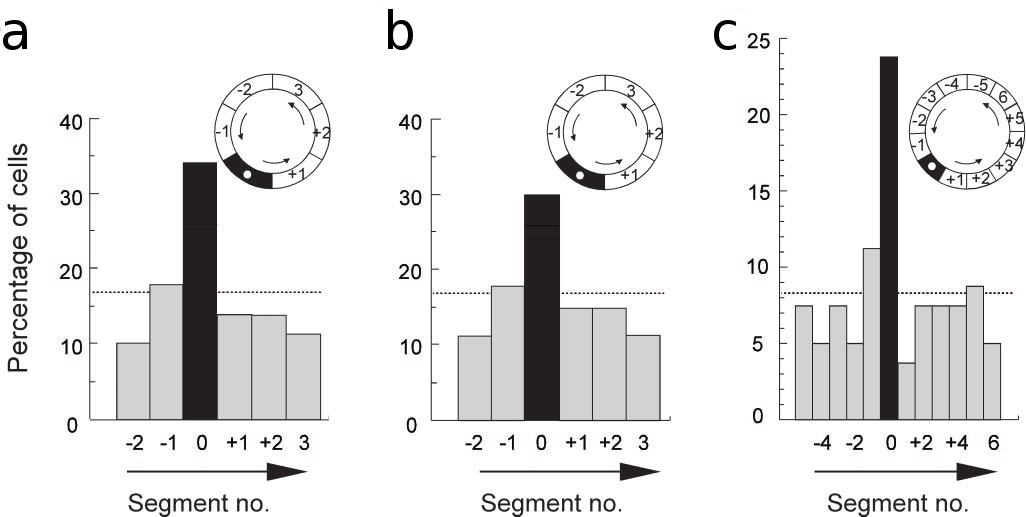
\includegraphics[width=0.7\textwidth]{intro/Hollup_accumulation_edit}
	\caption[Distribution of firing fields in Hollup et al.]{Distribution of firing fields in \citeauthor{Hollup2001a} after training with a constant platform location.
	\textbf{a}. Percentage of firing fields in each 60$^{\circ}$ segment of the corridor (80 cells; average of 3 probe tests). Field location was defined as the segment with the maximal averaged firing rate. Firing fields accumulated in the platform segment (segment 0, black). The chance level was at 16.7\%. Inset, Diagram of the corridor. Arrows indicate swim direction.
	\textbf{b}. Percentage of firing fields in each 60$^{\circ}$ segment after directional sorting (same trials and same symbols as described in \textit{a}). Only data sampled during swimming in the preferred direction are retained.
	\textbf{c}. Percentage of firing fields in segments of 30$^{\circ}$ after directional sorting. The platform was in the middle of segment 0.
	Reproduced from \citet{Hollup2001a}.}
	\label{fig:intro:memory:hollup}
\end{figure}

Conceptually similar, but drier, are the Barnes or cheeseboard maze \citep{Barnes1979, Kesner1991, Dupret2010a}.
These mazes consist of a large platform with holes throughout.
These holes can either be escapes that allow the mice/rats to avoid the exposed platform or baited/rewarded.
Either way, the degree of learning can be quantified by the latency to finding the correct location or the amount of time spent near previously rewarded locations during un-rewarded probe trials.
In a study by \citeauthor{Dupret2010a} which partially inspired my own work, the authors used a cheeseboard maze to examine hippocampal functional correlates of learning and memory (\citealp{Dupret2010a}; see \autoref{sec:df:methods:comp}).
The authors identified an increase in the fraction of hippocampal area CA1 place cells that encoded the reward location, the magnitude of which correlated with task performance (\autoref{fig:intro:memory:dupret}a,b).
In addition they found properties of \acp{SWR} that also correlated with task performance -- the fraction of pyramidal cells that participated in \ac{SWR} events during exploration (eSWRs) and the similarity of the pyramidal cell firing patterns during off-line \acp{SWR} (sSWRs) with on-line exploration of the reward locations (\autoref{fig:intro:memory:dupret}c,d).
In light of evidence pointing to a central role for SWRs in long-term memory consolidation \citep{Buzsaki2015}, it's tempting to interpret these findings as task performance being aided by an increased number of pyramidal cells encoding a memory of the reward locations during exploration and increased `remembering' of the rewarded locations during sleep.
In my own experiments, we found dysfunctional \ac{SWR} activity in mice that performed worse on our similar \ac{GOL} task, which aligns with these results (\autoref{sec:df:results:SWR}).

\begin{figure}
	\centering
	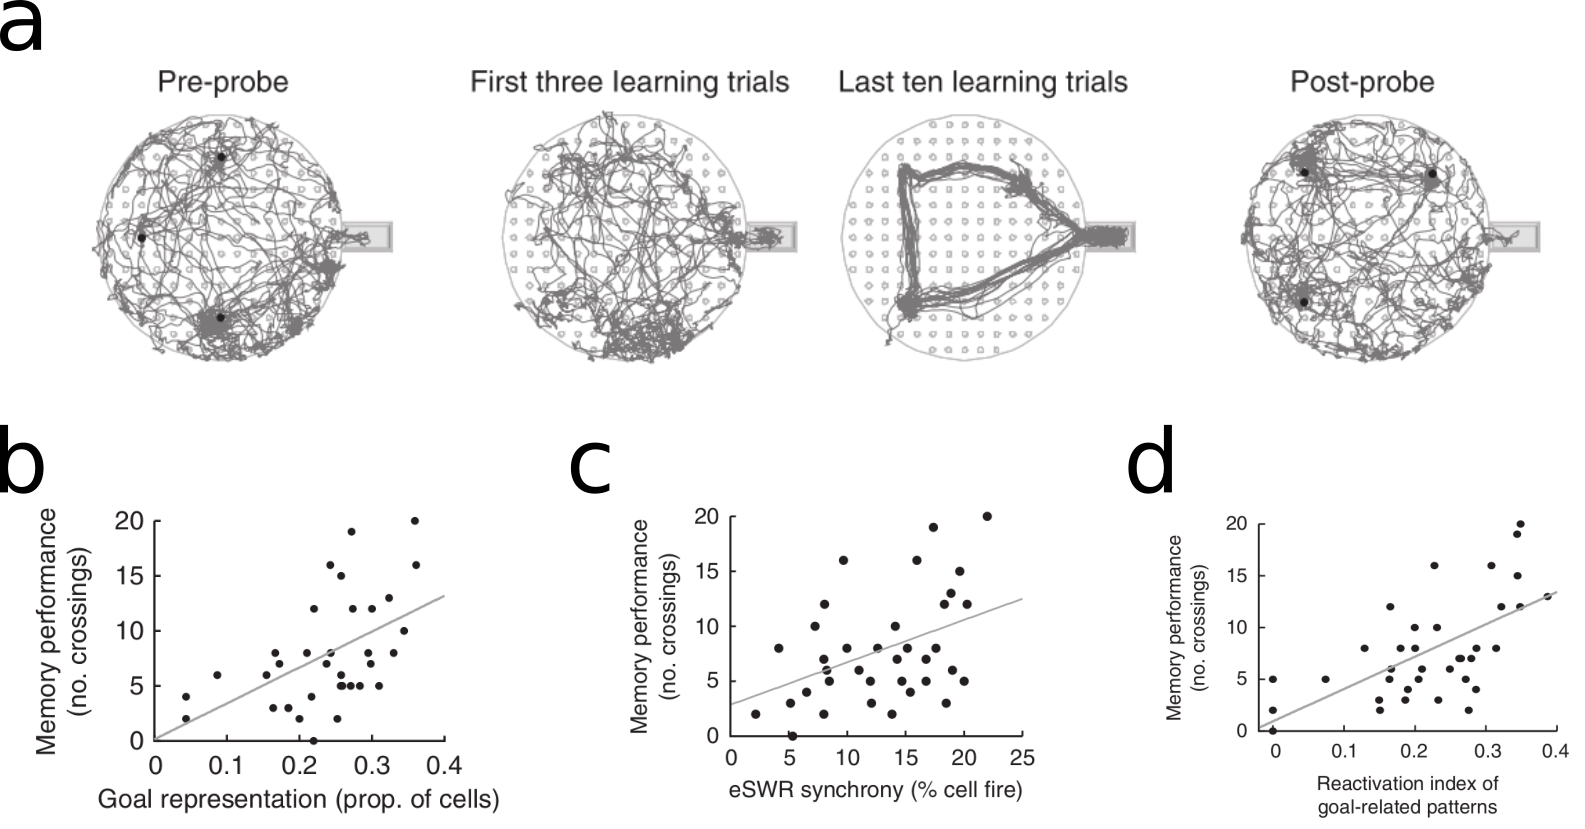
\includegraphics[width=0.7\textwidth]{intro/Dupret_cheeseboard_and_correlates}
	\caption[Cheeseboard task and behavioral correlates from Dupret et al.]{Cheeseboard task and behavioral correlates from Dupret et al.
	\textbf{a}. Representative examples of an animal's path; for clarity, only the first 10 min of each probe session is depicted (black dots, learnt goal locations).
	\textbf{b}. Scatter plot showing post-probe memory performance (number of crossings) as a function of the proportion of CA1 place cells at goal location during the end of learning (gray: regression line, r=0.511, P=0.0014).
	\textbf{c}. Scatter plot showing post-probe memory performance (number of crossings) as a function of `eSWR synchrony' (percentage of CA1 pyramidal cells that fire in eSWR) at the end of learning (gray: regression line, r=0.418, P=0.011).
	\textbf{d}. Scatter plot showing post-probe memory performance (number of crossings at a given goal location) as a function of the proportion of sSWRs in which assembly patterns represented the same goal location (gray: regression line, r=0.620, P=0.00005)
	Reproduced from \citet{Dupret2010a}.}
	\label{fig:intro:memory:dupret}
\end{figure}

\section{Memory in the brain}
\label{sec:intro:memory:structure}
The earliest behaviorist approaches to studying memory focused solely on the behavioral responses elicited by sensory inputs -- ignoring the `black box' that the brain was at the time \citep{Watson1913}.
It is now, perhaps obviously, recognized that behavioral responses intimately depend upon the organ that drives the response -- the brain.
The degree to which memory, and more generally cognitive functions, are localized within the brain has been widely debated.
In the late 1800's Pierre Paul Broca and Carl Wernicke identified patients with specific speech deficits related to the production and comprehension of language respectively.
These deficits were later found to be associated with specific lesions in the posterior inferior frontal gyrus and posterior section of the superior temporal gyrus, providing evidence for the localization of cognitive functions within the brain.
In contrast, work by Karl Lashley in the early 20\super{th} century showed that following the systematic removal of pieces of rat neocortex, performance in a previously-learned maze depended on the size of the lesion, but not the specific location \citep{Lashley1929}, lending support for the alternate \textsc{theory of mass action}.
Donald Hebb was one of the first to bring these two theories together, suggesting that networks of neurons could span many brain regions and collectively store memories \citep{Hebb1949}.

While circuits that perform many cognitive functions span the entire brain, there are also clearly cognitive functions that are localized to specific regions.
% While `memory' in it's broadest sense is a fundamental feature of every neuron, in mammals certain memory sub-types have been closely associated to specific brain regions.
For example, implicit procedural memory (e.g.~driving a car) is largely localized to the striatum and cerebellum \citep{Knowlton1996, Gerwig2007, Eichenbaum2000}, while emotional memory (e.g.~learned aversion) is largely attributed to the amygdala \citep{LeDoux2000}.
The neocortex is important for working memory, priming effects, and eventually the long-term storage of declarative memory.
While declarative memory may eventually be stored in the cortex, the \ac{HPC} is central to the process of consolidating declarative memories of experiences, and building association networks, such as in the case of spatial maps \citep{Eichenbaum2000}.
My primary research projects revolved around hippocampal-dependent spatial memory, so with no desire to minimize the important role of the rest of the brain in memory, I will focus on the \ac{HPC} for the remainder of this section. 

\subsection{The Hippocampus}
\label{sec:intro:memory:hpc}
The \ac{HPC} has been central to our study of memory at least since Scoville and Milner first reported in the 1950's on Henry Molaison (H.M.) who had profound anterograde amnesia following the bilateral removal of large portions of the medial temporal lobes, which includes the \ac{HPC} and parahippocampal structures \citep{Scoville1957}.
The most dramatic feature of H.M.'s memory loss was the inability to form new episodic memories, as he described it:
\begin{quote}
Every day is alone in itself, whatever enjoyment I've had, and whatever sorrow I've had.
\attrib{in \citealt{Milner1968}}
\end{quote}
Despite H.M.'s near complete inability to form new memories, he still maintained the ability to recall events from childhood and showed no general cognitive or intelligence decline \citep{Squire2009}.
% lending evidence to the idea of a distributed memory system, or at least separable facets of memory .
Additional studies of H.M. over the next 50 years revealed that while declarative memory deficits remained severely impaired, various forms of implicit memory remained unaffected \citep{Corkin2002}.
For example, patient H.M. was able to show day-to-day improvements in a mirror-tracing motor-learning task, despite no explicit memory of ever having performed the task before.
In addition, he showed normal word-list priming effects -- whereby words stems are preferentially completed by words semantically similar to recently viewed words. 
While the specific brain areas resectioned in the case of H.M. included structures adjacent to the \ac{HPC} as well (such as the amygdala), numerous studies have since shown that the \ac{HPC} in particular is essential for normal formation of long term episodic and semantic memory \citep[reviewed in][]{Eichenbaum2000, Burgess2002}.

\subsubsection{Circuitry of the \acl{HPC}}
The \acl{HPC} consists of the Ammons horn (Cornu Ammonis; CA) and \ac{DG}, which make up the \acl{HPC} proper, plus \ac{EC}, subiculum, presubiculum, and parasubiculum.
The CA regions contains three sequential subregions, spanning from the subiculum to the \ac{DG}; CA1, CA2, and CA3 \citep{deNo1934}.
The connectivity of the \ac{HPC} is one of the most well-characterized neuronal circuits within the mammalian brain.
Perhaps reflective of its fundamental role in memory processing, hippocampal-circuitry is also remarkably conserved across mammals \citep{Manns2006}.
The principal neurons in the \ac{HPC} communicate through the classically-defined trisynaptic loop: perforant path fibers project from layer II of the \ac{EC} to granule cells in the \ac{DG}, which in turn send mossy fiber projections to CA3 that finally project along the Schaffer collateral pathway and synapse upon proximal apical and basal dendrites of \acp{CA1PC}, which are the primary output node of the \ac{HPC}.
Among other projections to both cortical and subcortical structures, \acp{CA1PC} also send a projection back to deep layers of the \ac{EC}, completing the hippocampal loop.
In addition, layer II of \ac{EC} sends a direct perforant path projection to CA3 and layer III sends a direct projection through the temporoammonic pathway to distal dendrites of CA1.
CA2 receives direct inputs from CA3 and layer II neurons from lateral and medial \ac{EC}, and in turn send projections only within the \ac{HPC}, to CA3 and CA1 \citep{Hitti2014}. 
Large excitatory cells within the hilus (\textsc{mossy cells}) receive excitation from \ac{DG} granule cells and provide both direct feedback excitation and indirect feedback inhibition to granule cells (\citealp{Danielson2017}; \autoref{fig:intro:memory:HPC_circuitry}).
There are also reciprocal \acp{LRIP} between the \ac{EC} and CA1 that specifically target GABAergic \acp{IN} \citep{Melzer2012, Basu2016}.
% There are also long-range inhibitory projections (LRIP) from both medial and lateral \ac{EC} that targets inhibitory interneurons -- which in turn target CA1PC tuft dendrites -- near the \emph{stratum radiatum-stratum lacunosum moleculare} border in CA1 \citep{Basu2016}.
In \autoref{sec:other:LRIP}, I will discuss work I did characterizing the functional properties of the \ac{LRIP} from the \ac{EC} to CA1. 
% \todo[color=cyan, inline]{Brief overview of the hippocampal trisynaptic circuit. Hippocampal memory and navigation-related operations are thought to emanate from the trisynaptic circuitry residing in the hippocampus proper. SPELL OUT THE TRISYNAPTIC CIRCUTRY. "The hippocampal formation is comprised of the hippocampus proper or Ammon's horn (Cornu Ammonis; CA), as well as the \ac{DG}, \ac{EC}, parasubiculum, presubiculum and the subiculum. The hippocampus proper contains three discrete regions, designated CA1-3, stretching from subiculum to the \ac{DG}; the so-called CA4 area of Lorente de No (Ref) is now considered to be part of the \ac{DG} and called the hilus, and not regarded as a continuation of the PC layer. In the rat, the hippocampus contains approximately 311,500 CA1 and 204,700 CA3 PCs (Bezaire and Soltesz, 2013). The CA2 is a distinct, small region that is wedged between the CA3 and CA1 areas, with properties that in some but not all aspects resemble the part of the CA3 region immediately adjacent to it (Refs). The \ac{EC} provides the major excitatory input to the hippocampus, either to the \ac{DG} and the CA3 or to the CA1 and subiculum. The information flow carried by the excitatory connections between principal cells through the circuit of the hippocampal formation is primarily unidirectional, from the \ac{DG} to the CA3 and CA2, then to the CA1, subiculum and back to the entorhinal cortex."}
% \todo[color=cyan, inline]{LEC-MEC dual flow of information -- Knierim and Eichenbaum should be spelled out. Correct wording in the relevant section}
% Stellate Ocean cells in ECII project to the DG, CA3, and CA2 region, whereas ECIII cells directly project to the CA1 region. % Entorhinal–hippocampal neuronal circuits bridge temporally discontiguous events, Tonegawa

% \begin{figure}
% 	\centering
% 	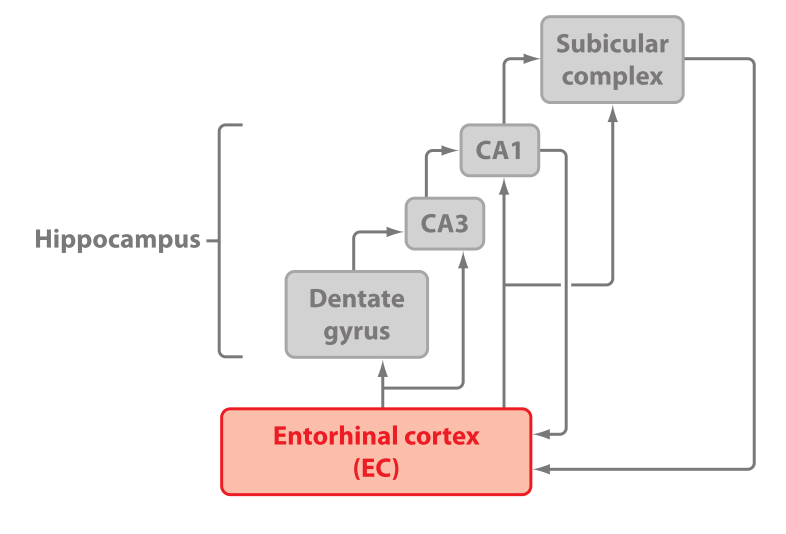
\includegraphics[width=0.5\textwidth]{intro/Squire2011_HPC_circuitry_edit}
% 	\caption[Schematic view of the medial temporal lobe memory system for declarative memory]{Schematic view of the medial temporal lobe memory system for declarative memory, which is composed of the hippocampus and the perirhinal, entorhinal, and parahippocampal cortices. In addition to the connections shown here, there are also weak projections from the perirhinal and parahippocampal cortices to the CA1-subiculum border.
% 	Reproduced from \citet{Squire2011}.}
% 	\label{fig:intro:memory:HPC_circuitry}
% \end{figure}
\begin{figure}
	\centering
	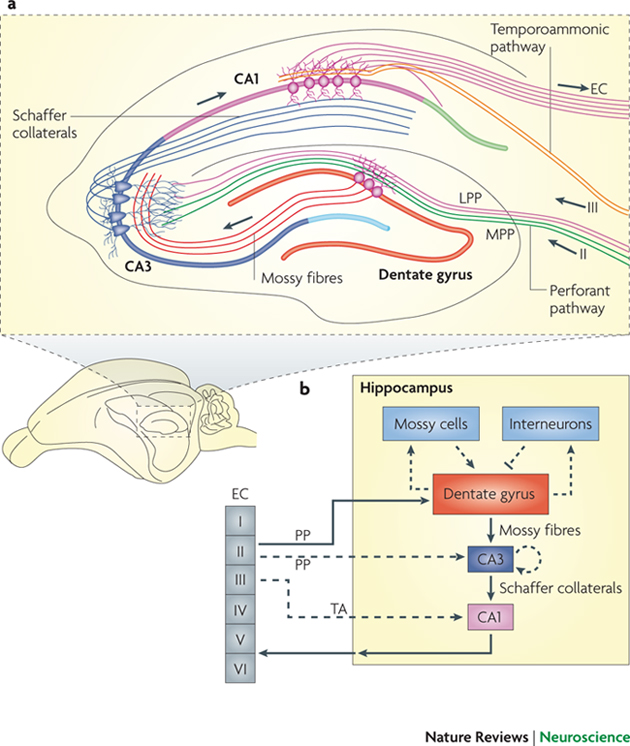
\includegraphics[width=0.7\textwidth]{intro/Deng2010_HPC_circuitry}
	\caption[The neural circuitry of the rodent \acl{HPC}]{The neural circuitry of the rodent \acl{HPC}.
	\textbf{a}. An illustration of the hippocampal circuitry.
	\textbf{b}. Diagram of the hippocampal neural network. The traditional excitatory trisynaptic pathway (\ac{EC}--\ac{DG}--CA3--CA1--\ac{EC}) is depicted by solid arrows. The axons of layer II neurons in the \ac{EC} project to the \ac{DG} through the perforant pathway (PP), including the lateral perforant pathway (LPP) and medial perforant pathway (MPP). The \ac{DG} sends projections to the pyramidal cells in CA3 through mossy fibers. CA3 pyramidal neurons relay the information to CA1 pyramidal neurons through Schaffer collaterals. CA1 pyramidal neurons send back-projections into deep-layer neurons of the \ac{EC}. CA3 also receives direct projections from \ac{EC} layer II neurons through the PP. CA1 receives direct input from EC layer III neurons through the temporoammonic pathway (TA). The dentate granule cells also project to the mossy cells in the hilus and hilar \acp{IN}, which send excitatory and inhibitory projections, respectively, back to the granule cells.
	Reproduced from \citet{Deng2010}.}
	\label{fig:intro:memory:HPC_circuitry}
\end{figure}

Finally, the \ac{HPC} is also targeted by afferents from neuromodulatory nuclei, including cholinergic and GABAergic projections from the medial septum  \citep{Klausberger2008}, serotonergic and glutamatergic projections from the raphe nuclei \citep{Varga2009}, as well as dopaminergic and noradrenergic projections from the ventral tegmental area \citep{Gasbarri1997} and locus coeruleus \citep{Foote1983}.

\subsubsection{Local \aclp{IN}}
\label{sec:intro:memory:INs}
The \ac{HPC} consists not only of a dense principal cell layer of excitatory pyramidal cells, but also diverse populations of local GABAergic \acp{IN} which control pyramidal cell spiking \citep{Freund1996}.
Classifications of \acp{IN} are generally determined by their unique neurochemical markers, morphological structure, location of the soma within the lamina of the \ac{HPC}, afferent connectivity, and target of inhibition.
Within area CA1 for example, at least 21 GABAergic \ac{IN} subtypes have been identified \citep{Klausberger2008}.
These can be broadly segregated into three functional categories based on their target: \textsc{dendrite-targeting}, \textsc{soma-targeting}, and \textsc{interneuron-targeting}.
The two main classes of pyramidal cell-targeting \acp{IN} -- dendrite-targeting (e.g.~somatostatin-positive; SST+) and soma-targeting (e.g.~parvalbumin-positive: PV+) \acp{IN} -- are uniquely situated to control different aspects of pyramidal cell activity.
Dendrite-targeting \acp{IN} can directly gate dendritic integration of inputs and have been shown to directly modulate pyramidal cell burst spiking \citep{Royer2012}.
Hippocampal-dendritic inhibition has also been implicated in efficient formation of contextual fear memories, work which I contributed to, but will not be discussing further \citep{Lovett-Barron2014}.
Soma-targeting \acp{IN} tightly control the output of hippocampal pyramidal cells, modulate theta-phase activity, and are robustly affected by behavioral state \citep{Klausberger2008, Lovett-Barron2012, Klausberger2003}.
Interneuron-targeting \acp{IN} generally express calretinin (CR) or vasointestinal peptide (VIP) and are located throughout the lamina of the \ac{HPC} \citep{Chamberland2012}.
Relatively less is known about their functional activity \emph{in vivo}, but their connectivity provides a dysnaptic disinhibitory drive to hippocampal pyramidal cells.
Local inhibition within the \ac{HPC} is essential for the normal control of network activity and the disruption of hippocampal GABAergic \acp{IN} has been linked to multiple psychological disorders \citep[reviewed in][]{Marin2012}, including \scz/ which I will discuss later (\autoref{sec:intro:scz:glutamate}).
% \todo[inline, color=cyan]{Include a section about GABAERGIC INs (perisomaic, dendrtic, disinhibitory) Somogyi Klausberger, Freund Buzsaki,}

\subsection{Functional organization of the \acl{HPC}}
As described above (\autoref{sec:intro:memory:hpc}), the \ac{HPC} is fundamental to our understanding of how the brain processes spatial and episodic memory, but it also plays an important role in emotion and anxiety-related behaviors \citep{Fanselow2010}.
The \ac{HPC} is essential in modulating the hypothalamic-pituitary-adrenal axis, as \ac{HPC} lesions disrupt the normal hormonal stress response \citep{Jacobson1991} and psychiatric disorders such as depression, posttraumatic stress disorder, and bipolar disorder, are associated with reduced \ac{HPC} volume \citep{Fanselow2010}.
These two cognitively distinct functions have been shown to segregate along the dorsal-ventral axis of the \ac{HPC}: \ac{dHPC} is associated with spatial and episodic memory and \ac{vHPC} with emotion, anxiety-related behaviors, social interaction, and fear \citep{Moser1998, Fanselow2010, Strange2014}.
Supporting this dissociation, lesions of \ac{dHPC}, but not \ac{vHPC}, impair performance in a Morris water maze test of spatial memory \citep{Moser1995} and taxi drivers recalling routes through a city show \ac{fMRI} activation of posterior \ac{HPC}, which corresponds to \ac{dHPC} in rodents \citep{Maguire1997}.
In contrast, lesions of \ac{vHPC} in rodents reduced innate fear responses as seen by increased time spent in the exposed arms of an elevated plus maze and affected the degree of social interaction \citep{Fanselow2010, Strange2014}.
More recently, \ac{vHPC} neurons have been shown to be active in social interaction experiments and reactivation of specific subsets showed memory retrieval and could be paired to an unconditioned stimulus \citep{Okuyama2016}.

In addition, the dorsal-ventral axis of the \ac{HPC} also correlates with gradients of both afferent and efferent connections.
Projections to the \ac{HPC}-proper from the \ac{EC} generally follow a mapping of the dorsal-ventral axis of the \ac{EC} to the dorsal-ventral axis of the \ac{HPC} \citep{Strange2014}.
Additionally, the return projections from area CA1 back to the \ac{HPC} follow the same mapping.
This spatial-segregation of projections also applies to the upstream cortical projections to the \ac{EC} which target specific dorsal-ventral locations such that brain regions more involved in spatial processing (such as the retrosplenial cortex) project to more dorsal \ac{EC} and regions more associated with emotion (such as the infralimbic cortex) project to more ventral \ac{EC} \citep{Strange2014}.
Output projections from area CA1 follow a similar pattern.
Dorsal \ac{HPC} preferentially projects to regions involved in navigation, such as the retrosplinial and anterior cingulate cortices, while uniquely-\ac{vHPC} projections target the olfactory bulb (which has been linked to depression), the amygdala, and the nucleus accumbens \citep{Moser1998, Fanselow2010, Strange2014}.
The anatomical connectivity listed above are examples of differential connectivity and certainly not an exhaustive list, but they do highlight the underlying anatomy that gives rise to the episodic memory-emotion dichotomy within the \ac{HPC}.

\subsubsection{Pyramidal cell functional diversity}
\label{sec:intro:memory:diversity}
% \todo[inline, color=cyan]{This is a bit out of the blue here. Again, it would be better if you had already introduced the general circuitry and which pyramidal cells you talk about here. In general, this section needs MORE work. You can start (and maybe name the chapter) of functional organization of the hippocampus; dorsal=spatial ventral=emotional, anxiety, fear, social, etc. AND THEN introduce the concept of heterogeneity along these axes.}
Beyond the overall organization along the dorsal-ventral axis of the \ac{HPC}, principal cells in the \ac{HPC} also vary in their genetic makeup, connectivity, and functional properties along the the transverse \citep{Igarashi2014} and radial \citep{Slomianka2011} axes as well.
In particular, the radial axis, which corresponds to neurodevelopmental age, can be divided into superficial and deep pyramidal cells with unique properties and connectivity \citep{Angevine1965, Schlessinger1978, Deguchi2011}. 
Deep pyramidal cells are generally larger, express \emph{Vipr2} and \emph{Sox5}, and they preferentially receive inputs from the septum and ventral striatum \citep{Nielsen2010, Sorensen1993, Sorensen1995}.
Functionally, they show more burst firing, and generally contain more spatial information, which reflects as a higher fraction of place cells \citep{Mizuseki2011}.
In contrast, superficial pyramidal cells are smaller, and express \emph{Calbindin-28k}, \emph{Zbtb20}, and \emph{Satb2} \citep{Sloviter1989, Slomianka1992}.
As part of my extended projects, I worked with colleagues to further characterize \emph{in vivo} functional properties and learning-related \emph{in vivo} dynamics of pyramidal cells along the radial axis (\autoref{sec:other:sf-deep}).

\subsubsection{Hippocampal computations}
\label{sec:intro:memory:hpc_comp}
Computational models of the \ac{HPC} have long posited that the \ac{EC}-\ac{DG}-CA3 circuit was well positioned anatomically to perform pattern separator/completion computations \citep{Marr1971, Treves1994, Knierim2016}.
The \ac{EC} to \ac{DG} connection is highly divergent, with 5 times as many \ac{DG} granule cells as \ac{EC} input cells \citep{Amaral1990}.
In addition, \ac{DG} granule cells are under heavy inhibitory control, as their very sparse activity has made them difficult to record from \emph{in vivo} and their activity seems to readily remap to context manipulations \citep{Neunuebel2014, Leutgeb2007}, perhaps the most direct measure of input decorrelation or \textsc{pattern separation} (\autoref{fig:intro:memory:subfield_IO}a).
Hippocampal area CA3 in comparison is most notably characterized by its dense recurrent connections between pyramidal cells which inspired the proposal of CA3 as a Hebbian autoassociation network \citep{Marr1971}.
Area CA3 receives excitatory inputs from both the strong `detonator' synapses of \ac{DG} granule cell Mossy fibers as well as perforant path inputs from the \ac{EC}.
These connections make the region much more excitable and are thought to support \textsc{pattern completion} (\autoref{fig:intro:memory:subfield_IO}b) by establishing attractor network dynamics that allows for the network to recall entire memories from partial cues \citep{Treves1992, Neunuebel2014}.
Finally, the CA1 output node of the \ac{HPC} has been suggested to play a role in novelty detection as a \textsc{comparator} \citep{Vinogradova2001, Lisman2001}, as it has access to both the internal \ac{HPC} processed information from CA3 Schaffer collaterals as well as direct temporoammonic path excitation from the \ac{EC} (\autoref{fig:intro:memory:subfield_IO}c).
% For CA1 novelty detectiojn, also:
% Conjunctive representations in learning and memory: Principles of cortical and hippocampal function.
% O'Reilly, Randall C.; Rudy, Jerry W.
% Psychological Review, Vol 108(2), Apr 2001, 311-345. http://dx.doi.org/10.1037/0033-295X.108.2.311
While the role of area CA2 has been historically understudied, recent work has elucidated an important role for CA2 in social memory \citep{Hitti2014}, aggression \citep{Wersinger2002}, and time coding \citep{Mankin2015}.

In addition to specialized functions for hippocampal subfields, specific input streams to the \ac{HPC} also serve distinct roles.
In particular, the temporoammonic path inputs to CA1 include both \ac{MEC} and \ac{LEC} projections which convey two distinct streams of information.
The \ac{MEC} projection is the primary spatial input to CA1 and conveys the `where' of an episodic memory.
In contrast, \ac{LEC} projections convey non-spatial, contextual and sensory information that contributes the `what' components of episodic memory \citep{Hargreaves2005, Dickerson2010, Eichenbaum2012}.
These two distinct input streams of spatial and non-spatial information also unequally project to CA1PC subpopulations (\autoref{sec:intro:memory:diversity}), with \ac{MEC} preferentially targeting proximal and deep \acp{CA1PC}, while \ac{LEC} preferentially projects to distal and superficial \acp{CA1PC} \citep{Masurkar2017}.
These inputs streams are not completely spatially separated, as within place cell populations differences in locations are encoded through global remapping and differences in context are encoded through rate remapping (see \autoref{sec:intro:memory:remapping}, \citealp{Leutgeb2005a}).
In agreement with this interpretation, the context-specific change in the active population of cells was impaired by lesions of \ac{LEC} \citep{Lu2013}.
Characterizing the \emph{in vivo} activity of the inhibitory component of the \ac{LEC} projection to CA1 was part of my work with collaborators that I will discuss briefly later (\autoref{sec:other:LRIP}).
% In addition, CA1 also receives neuromodulatory inputs and non-spatial, contextual inputs from LEC, and might provide the conjunctive spatial-contextual-salience output from the \ac{HPC}.
% \todo[color=cyan]{Alternatively is not the best here. `In addition' is good for the neuromodulatory inputs. BUT you need to be precise here about MEC and LEC: you have to introduce this in more precisely and more detail, what type of information they are thought to carry -- See Eichenbaum and Knierim reviews on "dual stream of information flow" (spatial non-spatial). Also FYI, Masurkar paper from Steve's lab} 

\begin{figure}
	\centering
	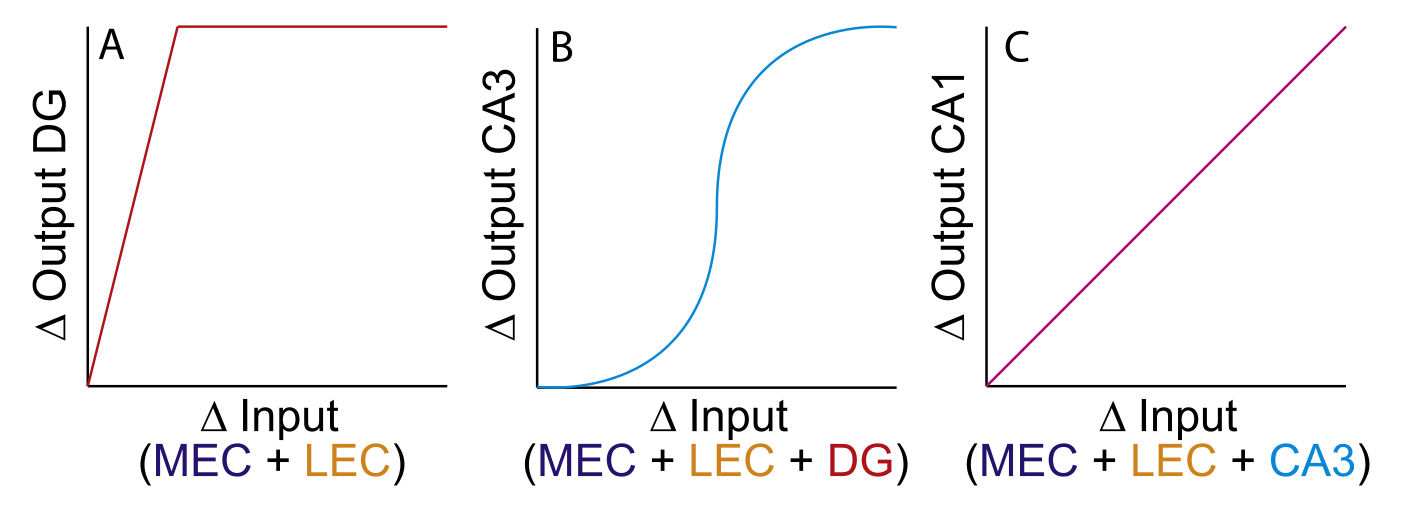
\includegraphics[width=0.8\textwidth]{intro/Knierim2016_subfield_IO_curves}
	\caption[Hypothesized input-output curves for the DG, CA3, and CA1 regions of the \acl{HPC}]{Hypothesized input-output curves for the DG, CA3, and CA1 regions of the \acl{HPC}. The $x$-axis of each graph denotes the difference between the neural activity representations of two specific input patterns. The $y$-axis represents the difference between the corresponding output patterns.
	\textbf{A}. The DG is hypothesized to change its output patterns to a greater extent than the input patterns change (pattern separation).
	\textbf{B}. CA3 is hypothesized to show a sigmoidal relationship between $\Delta$input and $\Delta$output, performing pattern completion with small $\Delta$input and pattern separation with large $\Delta$input.
	\textbf{C}. CA1 is hypothesized to display a linear relationship between $\Delta$input and $\Delta$output.
	Reproduced from \citet{Knierim2016}.}
	\label{fig:intro:memory:subfield_IO}
\end{figure}

% Burwell RD (2000): The parahippocampal region: Corticocortical connectivity. Ann N Y Acad Sci 911:25–42.
% \subsubsection{CA1}
% Pyramidal cells in hippocampal area CA1 are the principal excitatory neuron in that region and the primary output from the \ac{HPC}.
% \begin{figure}
% 	\centering
% 	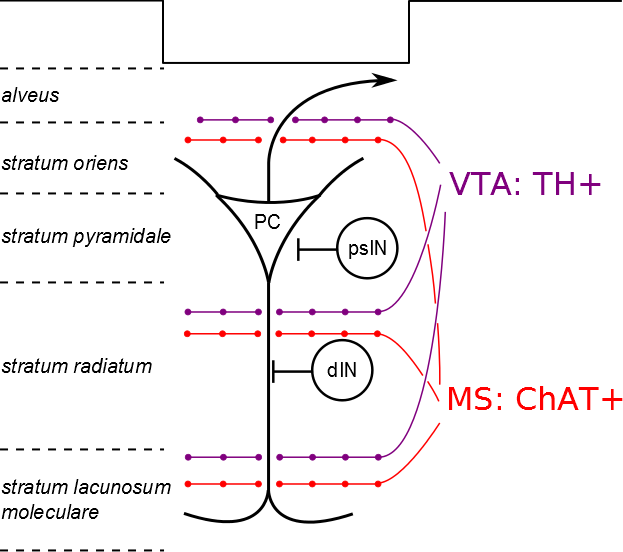
\includegraphics[width=0.5\textwidth]{intro/CA1-schematic_INs_VTA_MS}
% 	\caption{Schematic of major inputs to CA1 pyramidal cells}
% 	\label{fig:intro:memory:CA1_schematic}
% \end{figure}

\subsection{Memory at the synapse}

\subsubsection{Long-term potentiation}
\label{sec:intro:memory:LTP}
I have discussed the cognitive aspects of memory and the general brain regions involved, but what actually \textit{is} memory?
Mounting evidence over the years points to specific changes at the synapses between cells and the necessary molecular components that make this possible.
The search for memory in the brain is in fact the search for \textsc{hysteresis}, a dependence of the present activity of the brain on the past.
The first physiological example of this phenomenon in the brain was described by \citeauthor{Bliss1973} in 1973.
In anesthetized rabbits they found that high-frequency stimulation of the perforant path inputs to the \ac{HPC} resulted in the later enhancement of \ac{DG} granule population activity \citep{Bliss1973}.
This \ac{LTP} effect has now been studied extensively, with much of the work being done at two model synapses: the sensory- to motor-neuron synapse governing the siphon-withdrawal reflex of \emph{Aplysia californica} and synapses within the rodent \ac{HPC}, primarily the Schaffer collateral synapse from CA3 to CA1 \citep{Kandel2001, Bailey2008}.
In both \emph{Aplysia} and rodents, the molecular pathways giving rise to \ac{LTP} have been well established.
There are two primary stages of \ac{LTP}: early, short-term LTP (E-LTP) which involves modification of pre-existing proteins at the synapse, and late, long-term LTP (L-LTP) which involves new protein synthesis and potentially the formation of new synapses \citep{Frey1988, Bailey2008}.
These two distinct forms of LTP are reminiscent of short- and long-term memory, and have in fact been linked \citep{Moser1998a, Hernandez2008}, mostly through the shared-dependence on NMDA-receptors.
% \todo[color=red]{molecular LTP pathway, Kandel et al.}
% \citep{Frey1993} = cAMP/PKA role in L-LTP

\subsubsection{NMDA-receptor-dependent memory}
\label{sec:intro:memory:NMDAR}
Theoretical work had long posited that memory could be stored within neuronal networks by increasing the synaptic strengths between neurons that were active at the same time, effectively learning causal associations \citep{Hebb1949, Marr1971}.
The \ac{NMDAR}'s unique functional properties were recognized to make it will-suited as a coincidence detector.
Most essentially, the \ac{NMDAR} is blocked by magnesium in a voltage-dependent manner such that the block is released only when the postsynaptic neuron is depolarized, which when coupled with the \ac{NMDAR}'s slow activation and inactivation kinetics provides a time window for pre- and post-synaptic coincidence detection \citep[reviewed in][]{Bliss1993}.
In addition, \ac{NMDAR}s have high calcium permeability, allowing for their opening to trigger the influx of calcium that initiates the molecular pathway leading to \ac{LTP} \citep{Bailey2008}.

In the 1980's the study of acute hippocampal slices identified the \ac{NMDAR} -- an ionotropic glutamate receptor of which \ac{NMDA} is a selective agonist -- as being essential for the induction of \ac{LTP}, but not for normal synaptic transmission \citep{Collingridge1983}.
Richard Morris and colleagues were able to show that blocking \acs{NMDAR}s \emph{in vivo} with an intraventricular infusion of \ac{AP5} impaired mice on a spatial learning task \citep{Morris1986}.
These two findings together laid the foundation for future work which points towards an essential role for \ac{NMDAR}s in learning and memory \citep{Morris2013}.

Cloning of the genes for the \ac{NMDAR} subunits \citep{Moriyoshi1991} allowed for their detailed characterization and eventual mouse lines with the genes manipulated.
While global \emph{NR1}-knockout is lethal, mice were designed to selectively knockout \emph{NR1} in specific hippocampal subregions -- initially CA1 -- using the \emph{Cre/loxP} system which could be used to study the hippocampal-specific effect of \ac{NMDAR}s on memory \citep{Tsien1996}.
\citeauthor{Tsien1996} showed that CA1-specific knockout of \ac{NMDAR}s lead to impaired spatial memory in the hidden-platform water maze, but no impairment in the non-\acs{HPC}-dependent landmark task (where the reward is marked by a large proximal cue).
In addition, \ac{NMDAR}s have also been removed from the \ac{DG} \citep{McHugh2007} and CA3 \citep{Nakazawa2002} where deficits were observed in pattern separation and pattern completion/associative recall, respectively, suggesting that these two functions do in fact reside in the DG/CA3 regions and they involve active synaptic plasticity.
The selective removal of a single ion channel from single subregions of the \ac{HPC} strongly suggests an important role for hippocampal \ac{NMDAR}s and \ac{LTP}, and thus synaptic plasticity, in spatial learning and memory \citep{Tsien1996}.

% \citep[reviewed in][]{Nakazawa2004} for all
% \citep{Nakazawa2003} = CA3 NMDAR in one trial learning
% \citep{Brun2002} = separate CA3 and CA1, still see good place cells, can do spatial task, spatial recall impaired
% \citep{Hussaini2011} HCN1-KO mouse 

% \todo[inline, color=cyan]{INCOMPLETE  -- LTP and LTD should be all here from Bliss Lomo to date. This should be substantially expanded upon! 1) Section about LTP as a substrate of learning is critical. This should also encompass deficits of hippocampal learning, in particular spatial learning following NMDA KO (Nakazawa\&Tonegawa papers, 2002 Science, 2003 Neuron, review, Morris papers e.g. NMDA receptors and memory encoding, 2013) and CA3 and EC pathway manipulations  (Brun Sceince 2002)}

\section{Functional correlates of memory}
\label{sec:intro:memory:physiology}

% \subsection{Memory engrams}
% \todo[color=cyan]{Memory engrams section}
% Semon's orginal work and recent works by Josselyn (good review), Alcino Silva, Fankland, Tonegawa.
% In general this concept may worth a separate section in the introduction, including
% 1) the memory-based definition of engram. 
% 2) Recent IEG work attempting to "find" engram (NB: Peyman has been involved in Alcino Silva's recent engram studies, so questions related to engram stability and refining during CFC is likely) -see above. 
% 3) You can raise the disconnect between physiological studies of hippocampal learning-related population dynamics and the engram concept (the Josselyn review is very good on this)
% 4) This way you can get back to briefly in the conclusion and future directions at the end of thesis. 

\subsection{Spatial maps}
\label{sec:intro:memory:spatial_maps}
Perhaps the best-studied `engrams' in the mammalian brain are hippocampal place cells.
Throughout the \ac{HPC} (\ac{DG}, CA3, CA2, and CA1) there are principal cells that fire selectively at specific locations within an environment (\textsc{place cells}).
As an animal explores an environment these pyramidal cells show sparse spatially-modulated changes in firing rates that are established rapidly and subsequently remain stable \citep{O'Keefe1971, Thompson1990, Frank2004}.
These place cells form an allocentric map of the environment, which is essential for normal episodic memory function \citep{Smith2006c, Nakazawa2004, Buzsaki2013}.
Our understanding of place cells is a uniquely well-characterized functional mapping of the real world multiple synapses from both sensory and motor cortices.
In addition to place cells in the \ac{HPC}, the \ac{MEC} contains several categorized cell types involved in spatial navigation.
These include \textsc{grid cells}, which fire at regularly spaced intervals throughout an environment \citep{Hafting2005, Moser2014a}, head-direction cells \citep{Taube2007}, and border or boundary-vector cells, which fire at specific distances relative to the edges of an environment \citep{Solstad2008}.
Together with place cells, these cells collectively form the cellular foundation for the mammalian navigation system.

\begin{figure}
	\centering
	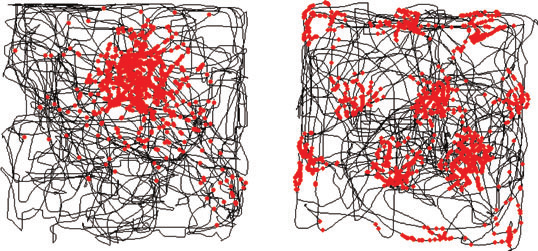
\includegraphics[width=0.7\textwidth]{intro/Moser_2008_place_grid}
	\caption[Place cell in the \acs{HPC} and grid cell in the \acs{MEC}]{Place cell in the \acs{HPC} \textit{a} and grid cell in the \acs{MEC} \textit{b}.
	Spike locations (\emph{red}) are superimposed on the animal's trajectory in the recording enclosure (\emph{black}).
	Whereas most place cells have a single firing location, the firing fields of a grid cell form a periodic triangular matrix tiling the entire environment available to the animal.
	Reproduced from \citet{Moser2008}.}
	\label{fig:intro:memory:place_grid}
\end{figure}

\subsubsection{Remapping}
\label{sec:intro:memory:remapping}
Place cells, like other forms of memory, are constantly trying to balance two competing constraints: on the one hand, their firing needs to be stable in order to be a helpful representation of the environment, but on the other hand, their firing needs to be plastic enough to constantly encode new environments, forget irrelevant information, and adapt to new features.
Place cells changing their firing properties to incorporate new features of the world is known as \textsc{remapping} \citep{Muller1987, Leutgeb2005a, Colgin2008}.
A given place cell is defined by it's spatial tuning -- it's place field -- and it's firing rate gain within the place field.
These seem to be independent factors, as either can remap separately.
\textsc{Global remapping} is the collective remapping of place field locations across a population of place cells.
Alternatively, \textsc{rate remapping} is a change in place field gain (the ratio of firing rate in to out of the place field), while place fields locations remain fixed.

Global remapping is generally triggered by discrete changes to environmental conditions \citep{Leutgeb2004, Leutgeb2005a}, but can also be triggered by particularly salient events \citep{Moita2004}.
The sudden and collective remapping of firing fields support the notion of place fields arising from discrete attractor states \citep{Jeffery2011a}, though the discreteness of the transition seems to depend on the specifics of the environmental manipulations \citep{Wills2005, Leutgeb2005b, Jezek2011}.
In contrast, rate remapping preserves firing fields (and grid cell firing), but the firing rate of place cells changes across the population.
This separation of position and rate coding has lead to the hypothesis that they code for spatial and episodic memory, respectively \citep{Leutgeb2005a}.
Indeed, while place field location is closely tied to grid cell activity in the medial entorhinal cortex, rate remapping depends specifically on lateral entorhinal inputs, which convey contextual information \citep{Lu2013}.
It is possible to observe incomplete remapping, known as \textsc{partial remapping}, though this generally refers to situations where subsets of cells respondent to alternate competing spatial reference frames \citep{Skaggs1998, Colgin2008}.

\subsubsection{Stability}
\label{sec:intro:memory:stability}
The complete population remapping of global remapping and the `rate-only' remapping of rate remapping do not tell a complete story of place fields firing dynamics.
More generally, the \textsc{stability} of place cells populations varies with elapsed time and environment novelty, is affected by neuromodulation, and differs by hippocampal subfield.
In area CA1, the place cell population changes over time, such that similarity of activity is greatest at short time scales and decays over time \citep{Mankin2012}.
In contrast, place cell firing is more stable over time in CA3, providing a means to both stably represent a given environment and also distinguish different experience by recency.
Place fields form rapidly ($<$10~min) and quickly stabilize \citep{Frank2004} and can remain stable for months with the right conditions \citep{Thompson1990, Lever2002a, Ziv2013}.
This long-term stability of place fields is both \ac{NMDAR}-dependent \citep{McHugh1996, Kentros1998} and requires new protein synthesis \citep{Agnihotri2004}, in a similar manner as LTP (\autoref{sec:intro:memory:LTP}) and other forms of declarative memory \citep{Hernandez2008}.

Several factors have additionally been shown to influence the stability of place cell tuning.
\citeauthor{Moita2004} trained mice in two chambers to establish separate place maps in both locations.
After becoming familiar to both, rats underwent a contextual fear conditioning protocol in one of the chambers, which selectively induced remapping in that one chamber, while place cells in the control chamber remained stable \citep{Moita2004}.
In addition, \citeauthor{Kentros2004} showed that increasing spatial saliences correlated with increased place field stability, and also showed that the stability could be modulated by systemic administration of dopamine D1/D5 receptor agonist/antagonists \citep{Kentros2004}, possibly through the dependence of CA1 LTP on D1/D5 receptor activity \citep{Huang1995}.
Place cell stability is a fundamental aspect of my main project (\autoref{ch:df}), as I also looked at place field stability as it relates to context novelty and task demands.
My main findings in wildtype mice agree with what was shown previously, but I also see disruptions in these normal stability mechanisms in \df/ mice.

\begin{figure}
	\centering
	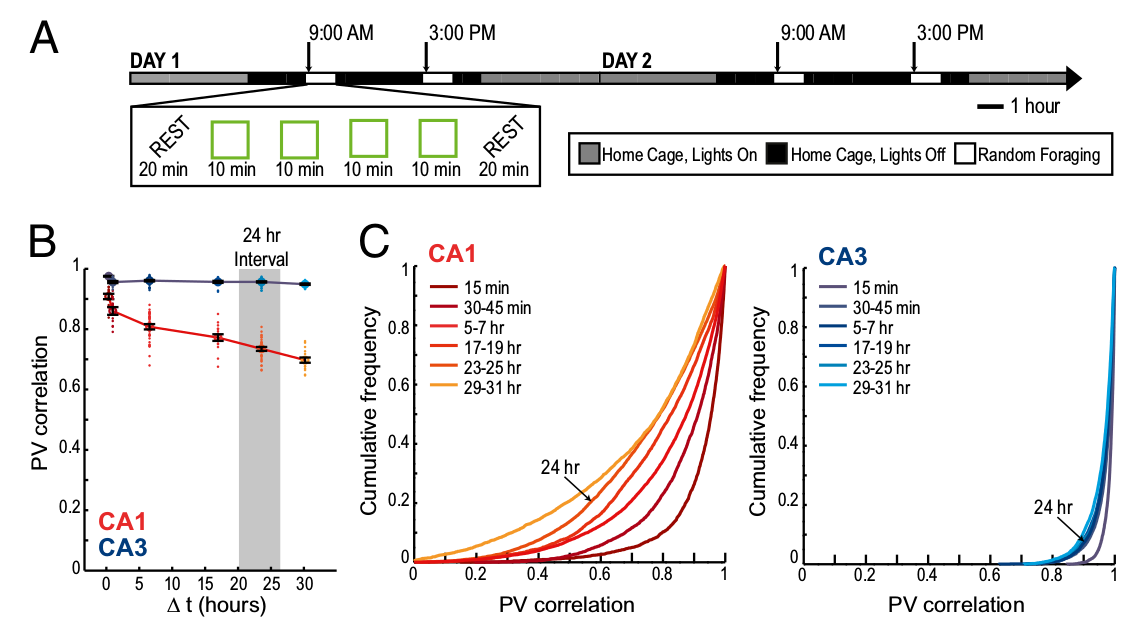
\includegraphics[width=0.8\textwidth]{intro/Mankin2012}
	\caption[Place cell population stability over days]{
		When testing with a single enclosure shape, firing patterns of the CA3 network remained highly consistent for repetitions of the same environment over extended time intervals, whereas activity patterns in the CA1 network changed.
		(A) An experimental design with a single enclosure shape.
		(B) PV correlations between pairs of recordings are shown as dots. The black error bars report the mean~$\pm$~SEM for pair-wise comparisons at each time interval.
		% The correlation coefficients for the CA1 population activity (red) decreased monotonically as a function of elapsed time between recording sessions up to at least 30~h.
		Highly consistent firing patterns in the CA3 population were observed over time intervals of 30~min to 30~h. In contrast, the CA1 network continued to show a pronounced monotonic decrease in firing similarity with time.
		(C) Cumulative distribution functions for PV correlations between pairs of recordings at different time intervals
	Reproduced from \citet{Mankin2012}.}
	\label{fig:intro:memory:time_stability}
\end{figure}

\section{Summary}
In summary, our memories are fundamental features of our identity.
We now are beginning to understand not just the cellular and circuit substrates for memory, but also the conditions that effect their formation and stability.
By expanding our knowledge of the basal brain state underlying memory, we can begin to understand not just the psychology of disrupted memory, but the actual cellular and circuit failures as well.
% \todo[color=cyan]{A better linking sentence would be good. This is an important part here where you are trying to link the work on basal/normal circuit to pathophysiology. You can use rely on some part of the main paper intro or discussion to expand upon this.}
In the next session I will discuss \scz/, and particularly how memory impairment is a core, debilitating symptom of the disease.
By better understanding the precise way in which memory fails, we can hope to find ways to help strengthen these memories, while at the same time also learn more about what is essential for the normal functioning of the declarative memory system.

\todo[color=cyan, inline]{I feel that a section "Modeling place cells dynamics" here about modeling place cell dynamics/remapping would work well here. You can this way: prep the reader for the modeiing chapter, summaize some previous work (Mehta, Hasselmo) on reward-related shift, Stress the importance of chronic cellular resolution recording to obain data for this. In general I would suggest to place more emphasis on this modeling -- both in the Introduction and in the conclusion section!!}
\todo[color=cyan, inline]{Phases of memory, consolidation -- model, role of SPW-R}